%Version 2.1 April 2023
% See section 11 of the User Manual for version history
%
%%%%%%%%%%%%%%%%%%%%%%%%%%%%%%%%%%%%%%%%%%%%%%%%%%%%%%%%%%%%%%%%%%%%%%
%%                                                                 %%
%% Please do not use \input{...} to include other tex files.       %%
%% Submit your LaTeX manuscript as one .tex document.              %%
%%                                                                 %%
%% All additional figures and files should be attached             %%
%% separately and not embedded in the \TeX\ document itself.       %%
%%                                                                 %%
%%%%%%%%%%%%%%%%%%%%%%%%%%%%%%%%%%%%%%%%%%%%%%%%%%%%%%%%%%%%%%%%%%%%%

%%\documentclass[referee,sn-basic]{sn-jnl}% referee option is meant for double line spacing

%%=======================================================%%
%% to print line numbers in the margin use lineno option %%
%%=======================================================%%

%%\documentclass[lineno,sn-basic]{sn-jnl}% Basic Springer Nature Reference Style/Chemistry Reference Style

%%======================================================%%
%% to compile with pdflatex/xelatex use pdflatex option %%
%%======================================================%%

%%\documentclass[pdflatex,sn-basic]{sn-jnl}% Basic Springer Nature Reference Style/Chemistry Reference Style


%%Note: the following reference styles support Namedate and Numbered referencing. By default the style follows the most common style. To switch between the options you can add or remove “Numbered” in the optional parenthesis. 
%%The option is available for: sn-basic.bst, sn-vancouver.bst, sn-chicago.bst, sn-mathphys.bst. %  
 
%%\documentclass[sn-nature]{sn-jnl}% Style for submissions to Nature Portfolio journals
%%\documentclass[sn-basic]{sn-jnl}% Basic Springer Nature Reference Style/Chemistry Reference Style
\documentclass[sn-mathphys,Numbered]{sn-jnl}% Math and Physical Sciences Reference Style
%%\documentclass[sn-aps]{sn-jnl}% American Physical Society (APS) Reference Style
%%\documentclass[sn-vancouver,Numbered]{sn-jnl}% Vancouver Reference Style
%%\documentclass[sn-apa]{sn-jnl}% APA Reference Style 
%%\documentclass[sn-chicago]{sn-jnl}% Chicago-based Humanities Reference Style
%%\documentclass[default]{sn-jnl}% Default
%%\documentclass[default,iicol]{sn-jnl}% Default with double column layout

%%%% Standard Packages
%%<additional latex packages if required can be included here>

\usepackage{graphicx}%
\usepackage{multirow}%
\usepackage{amsmath,amssymb,amsfonts}%
\usepackage{amsthm}%
\usepackage{mathrsfs}%
\usepackage[title]{appendix}%
\usepackage{xcolor}%
\usepackage{textcomp}%
\usepackage{manyfoot}%
\usepackage{booktabs}%
\usepackage{algorithm}%
\usepackage{algorithmicx}%
\usepackage{algpseudocode}%
\usepackage{listings}%
\usepackage{subfig}
\usepackage{float}
%%%%

%%%%%=============================================================================%%%%
%%%%  Remarks: This template is provided to aid authors with the preparation
%%%%  of original research articles intended for submission to journals published 
%%%%  by Springer Nature. The guidance has been prepared in partnership with 
%%%%  production teams to conform to Springer Nature technical requirements. 
%%%%  Editorial and presentation requirements differ among journal portfolios and 
%%%%  research disciplines. You may find sections in this template are irrelevant 
%%%%  to your work and are empowered to omit any such section if allowed by the 
%%%%  journal you intend to submit to. The submission guidelines and policies 
%%%%  of the journal take precedence. A detailed User Manual is available in the 
%%%%  template package for technical guidance.
%%%%%=============================================================================%%%%

%\jyear{2021}%

%% as per the requirement new theorem styles can be included as shown below
\theoremstyle{thmstyleone}%
\newtheorem{theorem}{Theorem}%  meant for continuous numbers
%%\newtheorem{theorem}{Theorem}[section]% meant for sectionwise numbers
%% optional argument [theorem] produces theorem numbering sequence instead of independent numbers for Proposition
\newtheorem{proposition}[theorem]{Proposition}% 
%%\newtheorem{proposition}{Proposition}% to get separate numbers for theorem and proposition etc.

\theoremstyle{thmstyletwo}%
\newtheorem{example}{Example}%
\newtheorem{remark}{Remark}%

\theoremstyle{thmstylethree}%
\newtheorem{definition}{Definition}%

\raggedbottom
%%\unnumbered% uncomment this for unnumbered level heads

\begin{document}

\title[Article Title]{HazeAway: A Convolutional Approach to Single-Image Haze Removal}

%%=============================================================%%
%% Prefix	-> \pfx{Dr}
%% GivenName	-> \fnm{Joergen W.}
%% Particle	-> \spfx{van der} -> surname prefix
%% FamilyName	-> \sur{Ploeg}
%% Suffix	-> \sfx{IV}
%% NatureName	-> \tanm{Poet Laureate} -> Title after name
%% Degrees	-> \dgr{MSc, PhD}
%% \author*[1,2]{\pfx{Dr} \fnm{Joergen W.} \spfx{van der} \sur{Ploeg} \sfx{IV} \tanm{Poet Laureate} 
%%                 \dgr{MSc, PhD}}\email{iauthor@gmail.com}
%%=============================================================%%

% \author[1]{\fnm{Mithun} \sur{Parab}}\email{mithun.sp@somaiya.edu}

% \author[2]{\fnm{Amisha} \sur{Bhanushali}}\email{bhanushali.amisha29@gmail.com}
% % \equalcont{These authors contributed equally to this work.}

% \author[3]{\fnm{Palash} \sur{Ingle}}\email{palash@sju.ac.kr}

% \author[4]{\fnm{Bharatesh} \sur{Chakravarthi}}\email{chakravarthi589@gmail.com}
% \author[5]{\fnm{Prabhu Prasad} \sur{B M}}\email{prabhuprasad1990@gmail.com}

% \author[6]{\fnm{Pavan Kumar} \sur{B N}}\email{pavanbn8@gmail.com}

% \equalcont{These authors contributed equally to this work.}

% H.S.V.P.S. R.J. College, Mumbai, India
% Sejong University, Seoul, South Korea
% Active Perception Group, School of Computing and Augmented Intelligence, Arizona State University, USA
% CSE Group, Indian institute of information technology, Sri city, India

% \affil[1]{ \orgname{H.S.V.P.S. R.J. College}, \city{Mumbai}, \country{India}}

% \affil[2, 3]{ \orgname{Sejong University}, \city{Seoul}, \country{South Korea}}

% \affil[4]{\orgdiv{Active Perception Group, School of Computing and Augmented Intelligence,} \orgname{Arizona State University},\country{USA}}

% \affil[5]{\orgdiv{Department of CSE} \orgname{Indian Institute of Information Technology}, \city{Dharwad}, \country{India}}

% \affil[6]{\orgdiv{CSE Group} \orgname{Indian Institute of Information Technology}, \city{Sri city}, \country{India}}

% \affil[2, 3]{\orgdiv{Department}, \orgname{Organization}, \orgaddress{\street{Street}, \city{City}, \postcode{10587}, \state{State}, \country{Country}}}

% \affil[4]{\orgdiv{Department}, \orgname{Organization}, \orgaddress{\street{Street}, \city{City}, \postcode{610101}, \state{State}, \country{Country}}}

% old eg.
% \affil[4]{\orgdiv{Department}, \orgname{Organization}, \orgaddress{\street{Street}, \city{City}, \postcode{610101}, \state{State}, \country{Country}}}

%%==================================%%
%% sample for unstructured abstract %%
%%==================================%%

\abstract{The existence of particles in the air cause haze, and this haze or fog cause degraded visibility in the captured shot from the camera. The non-uniform distribution of these particles, along with smoke, low light and pollution in the atmosphere, makes haze removal difficult in the real world images. The core computer vision tasks struggle with hazy images due to the lack of detail and poor visibility. The existing method relies on a transmission map in amalgamation with the atmospheric scattering input images to reconstruct a haze-free depiction. We suggested a single-image convolutions neural network that removes the haze present in the image and improves the perceptual quality by enhancing visibility. We used U-Net-like architecture with an encoder, bottleneck and decoder coupled with skip connections. In our experiment, we demonstrated the results on various benchmark dataset and compared our results with existing approaches. Additionally we compared the results from our network training on different image representations RGB verses YCbCr. The proposed method is straightforward and miniature yet still gives near state-of-the-art results.}

%%================================%%
%% Sample for structured abstract %%
%%================================%%

% \abstract{\textbf{Purpose:} The abstract serves both as a general introduction to the topic and as a brief, non-technical summary of the main results and their implications. The abstract must not include subheadings (unless expressly permitted in the journal's Instructions to Authors), equations or citations. As a guide the abstract should not exceed 200 words. Most journals do not set a hard limit however authors are advised to check the author instructions for the journal they are submitting to.
% 
% \textbf{Methods:} The abstract serves both as a general introduction to the topic and as a brief, non-technical summary of the main results and their implications. The abstract must not include subheadings (unless expressly permitted in the journal's Instructions to Authors), equations or citations. As a guide the abstract should not exceed 200 words. Most journals do not set a hard limit however authors are advised to check the author instructions for the journal they are submitting to.
% 
% \textbf{Results:} The abstract serves both as a general introduction to the topic and as a brief, non-technical summary of the main results and their implications. The abstract must not include subheadings (unless expressly permitted in the journal's Instructions to Authors), equations or citations. As a guide the abstract should not exceed 200 words. Most journals do not set a hard limit however authors are advised to check the author instructions for the journal they are submitting to.
% 
% \textbf{Conclusion:} The abstract serves both as a general introduction to the topic and as a brief, non-technical summary of the main results and their implications. The abstract must not include subheadings (unless expressly permitted in the journal's Instructions to Authors), equations or citations. As a guide the abstract should not exceed 200 words. Most journals do not set a hard limit however authors are advised to check the author instructions for the journal they are submitting to.}

\keywords{Haze removal, De-hazing, U-Net, Visibility enhancement, Convolution neural networks.}

%%\pacs[JEL Classification]{D8, H51}

%%\pacs[MSC Classification]{35A01, 65L10, 65L12, 65L20, 65L70}

\maketitle

\section{Introduction}
\label{introduction}
The light disperses into the surroundings, or it gets absorbed by the fragments present in the airspace. The total amount of fragments in the region is proportional to the scattering of light. This scattering reduces the clarity and colour in that region. Different particles and the environment they are in impact the scattering. Such as humidity and particles like sulphur cause a hazier environment. Most of these particles are present due to air pollution from industry. Some exist because of the natural world, such as windblown dust and forest fire. This haze, coupled with smoke, dust and low light condition, makes the haze removal task particularly difficult. This haze makes visibility extremely difficult for both humans and computer vision. e.g. the analysis from Wang et al. \cite{tourist}  concluded, the presence of haze can drastically effects tourist arrival. For better and more effective accuracy, vision algorithms expect clean, clear, and visible input. Since real-world places have haze environment tasks like object detection \cite{obj_det_cnn}, object segmentation \cite{motion_seg_cnn} becomes difficult due to a lack of information in captured images. To get the best out of these algorithms, we need to process real-world data to have the minimum possible haze and other artefacts. We can fix this via either pre-processing,  post-processing or both. Haze removal could be achievable in two ways physical and non-physical. The physical method analyses the atmospheric transmission that degrades the image and regenerates the image by inversing the existing transmission. The physical-based methods take the path of approximation and assumption about the prior condition. The non-physical-based techniques solve this problem through image enhancement. Popular approaches like Histogram equalization \cite{lai}, logarithmic transformation \cite{multi_sc}, various filters \cite{filters, pol_fil_sc, pol_filter2, prior_filt} in the frequency domain and Retinex theory \cite{retinex} are very robust and achieve remarkable results. These methods are not robust to the change and thus struggle with noise, different exposure settings and artefacts in the image. The core computer vision task needs clean and visible input to give a decent performance. Tasks like object detection, segmentation, and depth estimation deal with real-world data, these tasks struggle in performance when the images are hazy. We present a simple and miniature method to pre-process the input image, such that the performance of these tasks will improve.
\\
Recently, Deep learning-based methods perform exceptionally on the image enhancement task. These methods provide robust solutions to haze removal better than the quaint algorithm results. In this paper, we remove haze from both indoor and outdoor images. Our methods fix the different difficulties in the real world of hazy images like noise, challenging light and image artefacts. We constructed U-Net-like CNN \cite{u_net} with an encoder, bottleneck and decoder. Each of these consists of blocks of layers carefully designed for haze removal. These blocks consist of downsampling and upsampling layers with skip connections. We used a combination of loss functions to enhance different aspects of the images like the structural and perceptual quality of the image.
\\
The outline of the paper is summarized as follows. In this Section \ref{introduction}, we described haze and the difficulties faced in the haze removal process. Also, we explained the goal of the suggested method. In Section \ref{related_work}, we will discuss existing literature, the popular methods and their approach to solving the haze removal problem. The proposed technique and details about the model architecture and implementation are in Section \ref{proposed_method}. Training structure and comparison of our results with different methods are illustrated Section \ref{experiments}. Finally in Section \ref{conclusion}, we concluded the findings and summarised our approach of single image haze removal.
\section{Related Work}
\label{related_work}
We can categorise haze removal tasks into prior-knowledge and learning-based techniques. The prior-knowledge approaches take advantage of statistical hypotheses. In opposition, learning-based methods learn the nonlinear mapping in the  haze-free and between the given haze-full image. This section, we will embrace the difference between these two techniques in detail. In the prior-based algorithms \cite{prior_cap, prior_filt}, physical assumptions such as atmospheric scattering technique (ATM)   \cite{atm, real_time_atm, atm_illu} and statistical hypotheses are used to expect the outcome to be a haze-free image.
In the prior-based methods \cite{prior1, prior2, prior_cap, prior_cnn1, prior_filt}, authors investigate the factors affecting the image and minimize those factors to get a haze-free outcome. The transmission map with colour attenuation prior is calculated to manipulate the discrepancy between RGB channels. However, these techniques only reach sub-optimal performance in haze removal. Other approaches include polarized filters, multiview images of the common scenery and prior-based hazy methods. He et al. demonstrated dark channels prior (DHCP) \cite{he} to improve visibility in haze-full images. This approach struggles with edge structure and undergoes a halo effect \cite{halo_cai_cnn}. Further approaches Lai et al. \cite{lai} proposed two prior-based transmission maps for the hazy scene, a multi-scale retinex-based algorithm \cite{wang} to estimate luminous detail in the image, colour attenuation prior (CAP) \cite{prior_cap}, and an HSV colourspace method to extract haze-related features. 
\\
In learning-based methods, the first few techniques estimated transmission maps using end-to-end CNN like Cai et al.\cite{halo_cai_cnn} and Ren et al. \cite{ren} Zhang et al. \cite{zhang} suggested an approach to get transmission maps and atmospheric light with atmospheric scattering to estimate haze-free images. A variety of methods used CNN \cite{prior_cnn1, cnn_o, obj_det_cnn, halo_cai_cnn} to get a direct clean haze-free image. The result of the investigation from Chen et al. \cite{gated} using dilated convolutional for haze-free image reconstruction showed better unit performance than the previous existing methods.The approaches like AOD-net \cite{aod} analyzes the contradiction between the  quaint atmospheric models and the haze removal techniques. Later Swami et al. \cite{swami} proposed conditional GAN to remove haze from the degraded hazy images. Now, researchers \cite{res_unp, res_unp1} use an unpaired training approach for a variety of computer vision tasks. Various methods used this unpaired training technique some even used this for motion object segmentation \cite{motion_seg_cnn}. Another application-specific task on haze removal includes Chen et al. \cite{non_uniform} proposed nonuniform remote sensing technique for removing the haze. Zheng et al. \cite{uhd} performed dehazing on a Ultra-high definition image   using multi-guided bilateral learning. Illumination adjustment for haze \cite{col_d_ill}, smoke and fire removal from a single input image. VRHI \cite{VRHI} is used for visibility restoration in hazy images by incorporating haze density model. 
\\
In GAN-based techniques \cite{multi_scale_ad}, BPPnet \cite{bppnet_sota} used a pyramid-based network that gives state-of-the-art results with only 20 pairs of training images. EDN-GTM \cite{sec_sota} use dark channel prior in their approach with a guided transmission map that outperforms the traditional methodology. DW-GAN \cite{dw_gan} used discrete wavelet transform with two-branch GAN. RI-GAN \cite{ri_gan} with residual inception modules in both generator and discriminator. All of the above-mentioned methods works decently on haze removal task, but the GANs are computationally expensive and difficult to implement. Therefore, our model is CNN-based, easy to implement and computationally inexpensive.
\section{Proposed Method}
\label{proposed_method}
% In this Section, we will discuss our complete architecture. But first, we will examine the analysis of different colourspace image representations for the haze removal task. Then we will present the detail about the architecture of the proposed model with an overview of the model. In the end different losses and metrics and their influence on the proposed network will be present.

 \begin{figure*}[ht]
    \centering
    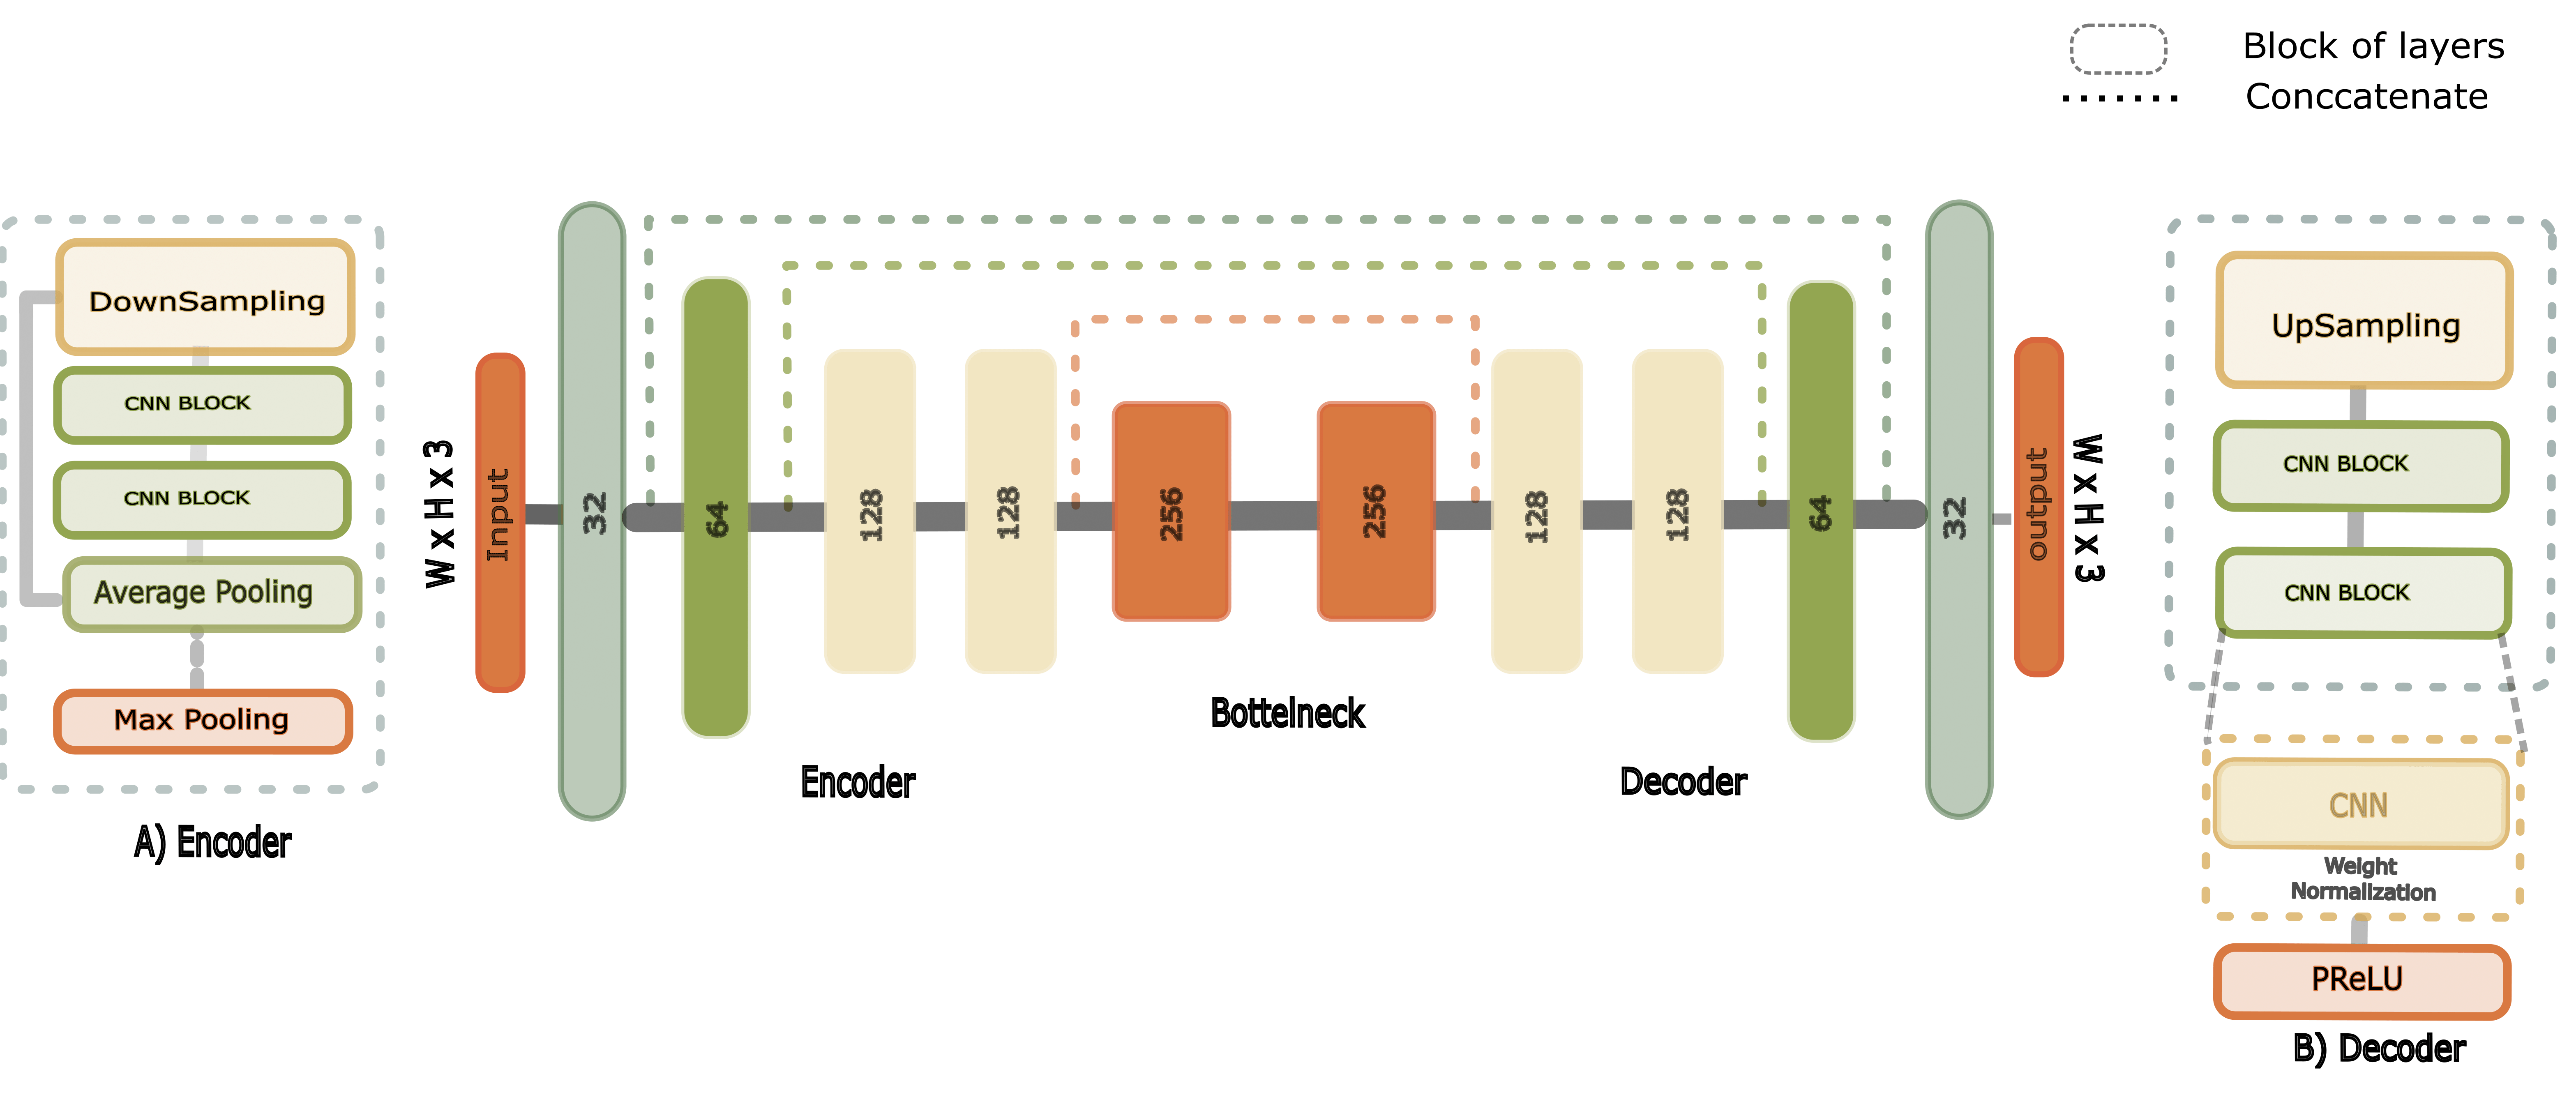
\includegraphics[height=0.5\textwidth, width=0.99\textwidth]{images/i4c_haze.png}
    \caption{The architecture we used in this paper for haze removal. A) Encoder block and B) Decoder block}
    \label{fig:haze_removal_model}
\end{figure*}
\subsection{Colour space}\label{color_space}
We compared RGB and YCbCr colourspace as training inputs to our neural network. We determined that the YCbCr image representation works very well on image haze removal. The YCbCr colourspace is mainly used in image enhancement and image super-resolution tasks because it represents information better than RGB and is noise free compared to RGB colourspace. Recently, YCbCr image representation has shown exceptional outcomes in haze removal tasks. 
As Bianco et al. \cite{hr_haze} showed in their experiment, the mean squared error \textit{(MSE)} \eqref{eqn:mse} is qualitatively better in YCbCr colourspace than RGB because atmospheric illumination in hazy images affects more Y channel more. A better \textit{MSE}  score in YCbCr colourspace is the direct reason for better peak-signal-to-noise ratio \textit{(PSNR)}. Therefore to evaluate the methodology, we will be using YCbCr colourspace as our primary image input representation.
\subsection{Model overview}\label{model_overview}
We prioritise performance, efficiency and simple architecture for our neural network model. The proposed technique is miniature and straightforward to conduct yet achieves better performance than the traditional methodology. We experimented with different approaches that will advance our expectations from our model. The proposed architecture is a U-Net-based formation of encoder, bottleneck and decoder. Each of the sub-formations is a set of cautiously selected blocks of layers that meet close to our prioritise. 
\\
Our end-to-end network's encoder and decoder are composed of convolutional blocks. Each of these blocks contains manually designed layers. Such as the encoder is constructed of downsampling layers and convolutional layers with pre-defined pooling. Whereas the decoder is created using upsampling layers and convolutional layers. These blocks coupled with the skip connection make our network end-to-end. We avoided the batch-normalization layer because of its poor performance on small batches, expensive computation and dissimilarity between training and testing. We used weight normalization because of is computationally inexpensive and gives better weight initialization. We used parametric  PReLU as our activation function since PReLU's learn parameters on how activation should be permitted for negative values.The bottleneck is created with only convolutional layers with fixed weights and biases. 
\subsection{Model architecture}\label{model_arch}
As outlined in Fig \eqref{fig:haze_removal_model}, the encoder is stacked with multiple convolutional blocks. Each of these blocks contains a set of convolutional layers, average pooling, max pooling, weight normalization and parametric ReLU. We downsampled the input by half i.e. the stride of two and raise the weight by a factor of two. The feature extracted in the block passed to the next block till they reach the bottleneck. The encoder is directly connected to the decoder via skip connection. Such that, the initially learned parameter could directly transfer to the decoder. The bottleneck is the only phase without any skip connection and sampling.  The input and output size of this phase is equal and the weight is the same for each block. 
\\
The decoder is composed of downsampling convolutional blocks. The decoder has the same set of layers as the encoder except for the downsampling layers such as average pooling and max pooling decoder has an upsampling layer. we used stride two with decreasing weight by a factor of two. For upsampling, we used bilinear interpolation. The decoder is directly connected to encode via skip connections from which the decoder gets learned parameters from an encoder.


\begin{figure*}[ht]
\caption{The results on datasets O-Haze \cite{o_haze} and I-Haze \cite{i_haze}}
\centering
\begin{tabular}{ccc}
Ground-truth  & \multicolumn{1}{c}{Input} & \multicolumn{1}{c}{ Our } \\
 \subfloat[]{\label{set5-original}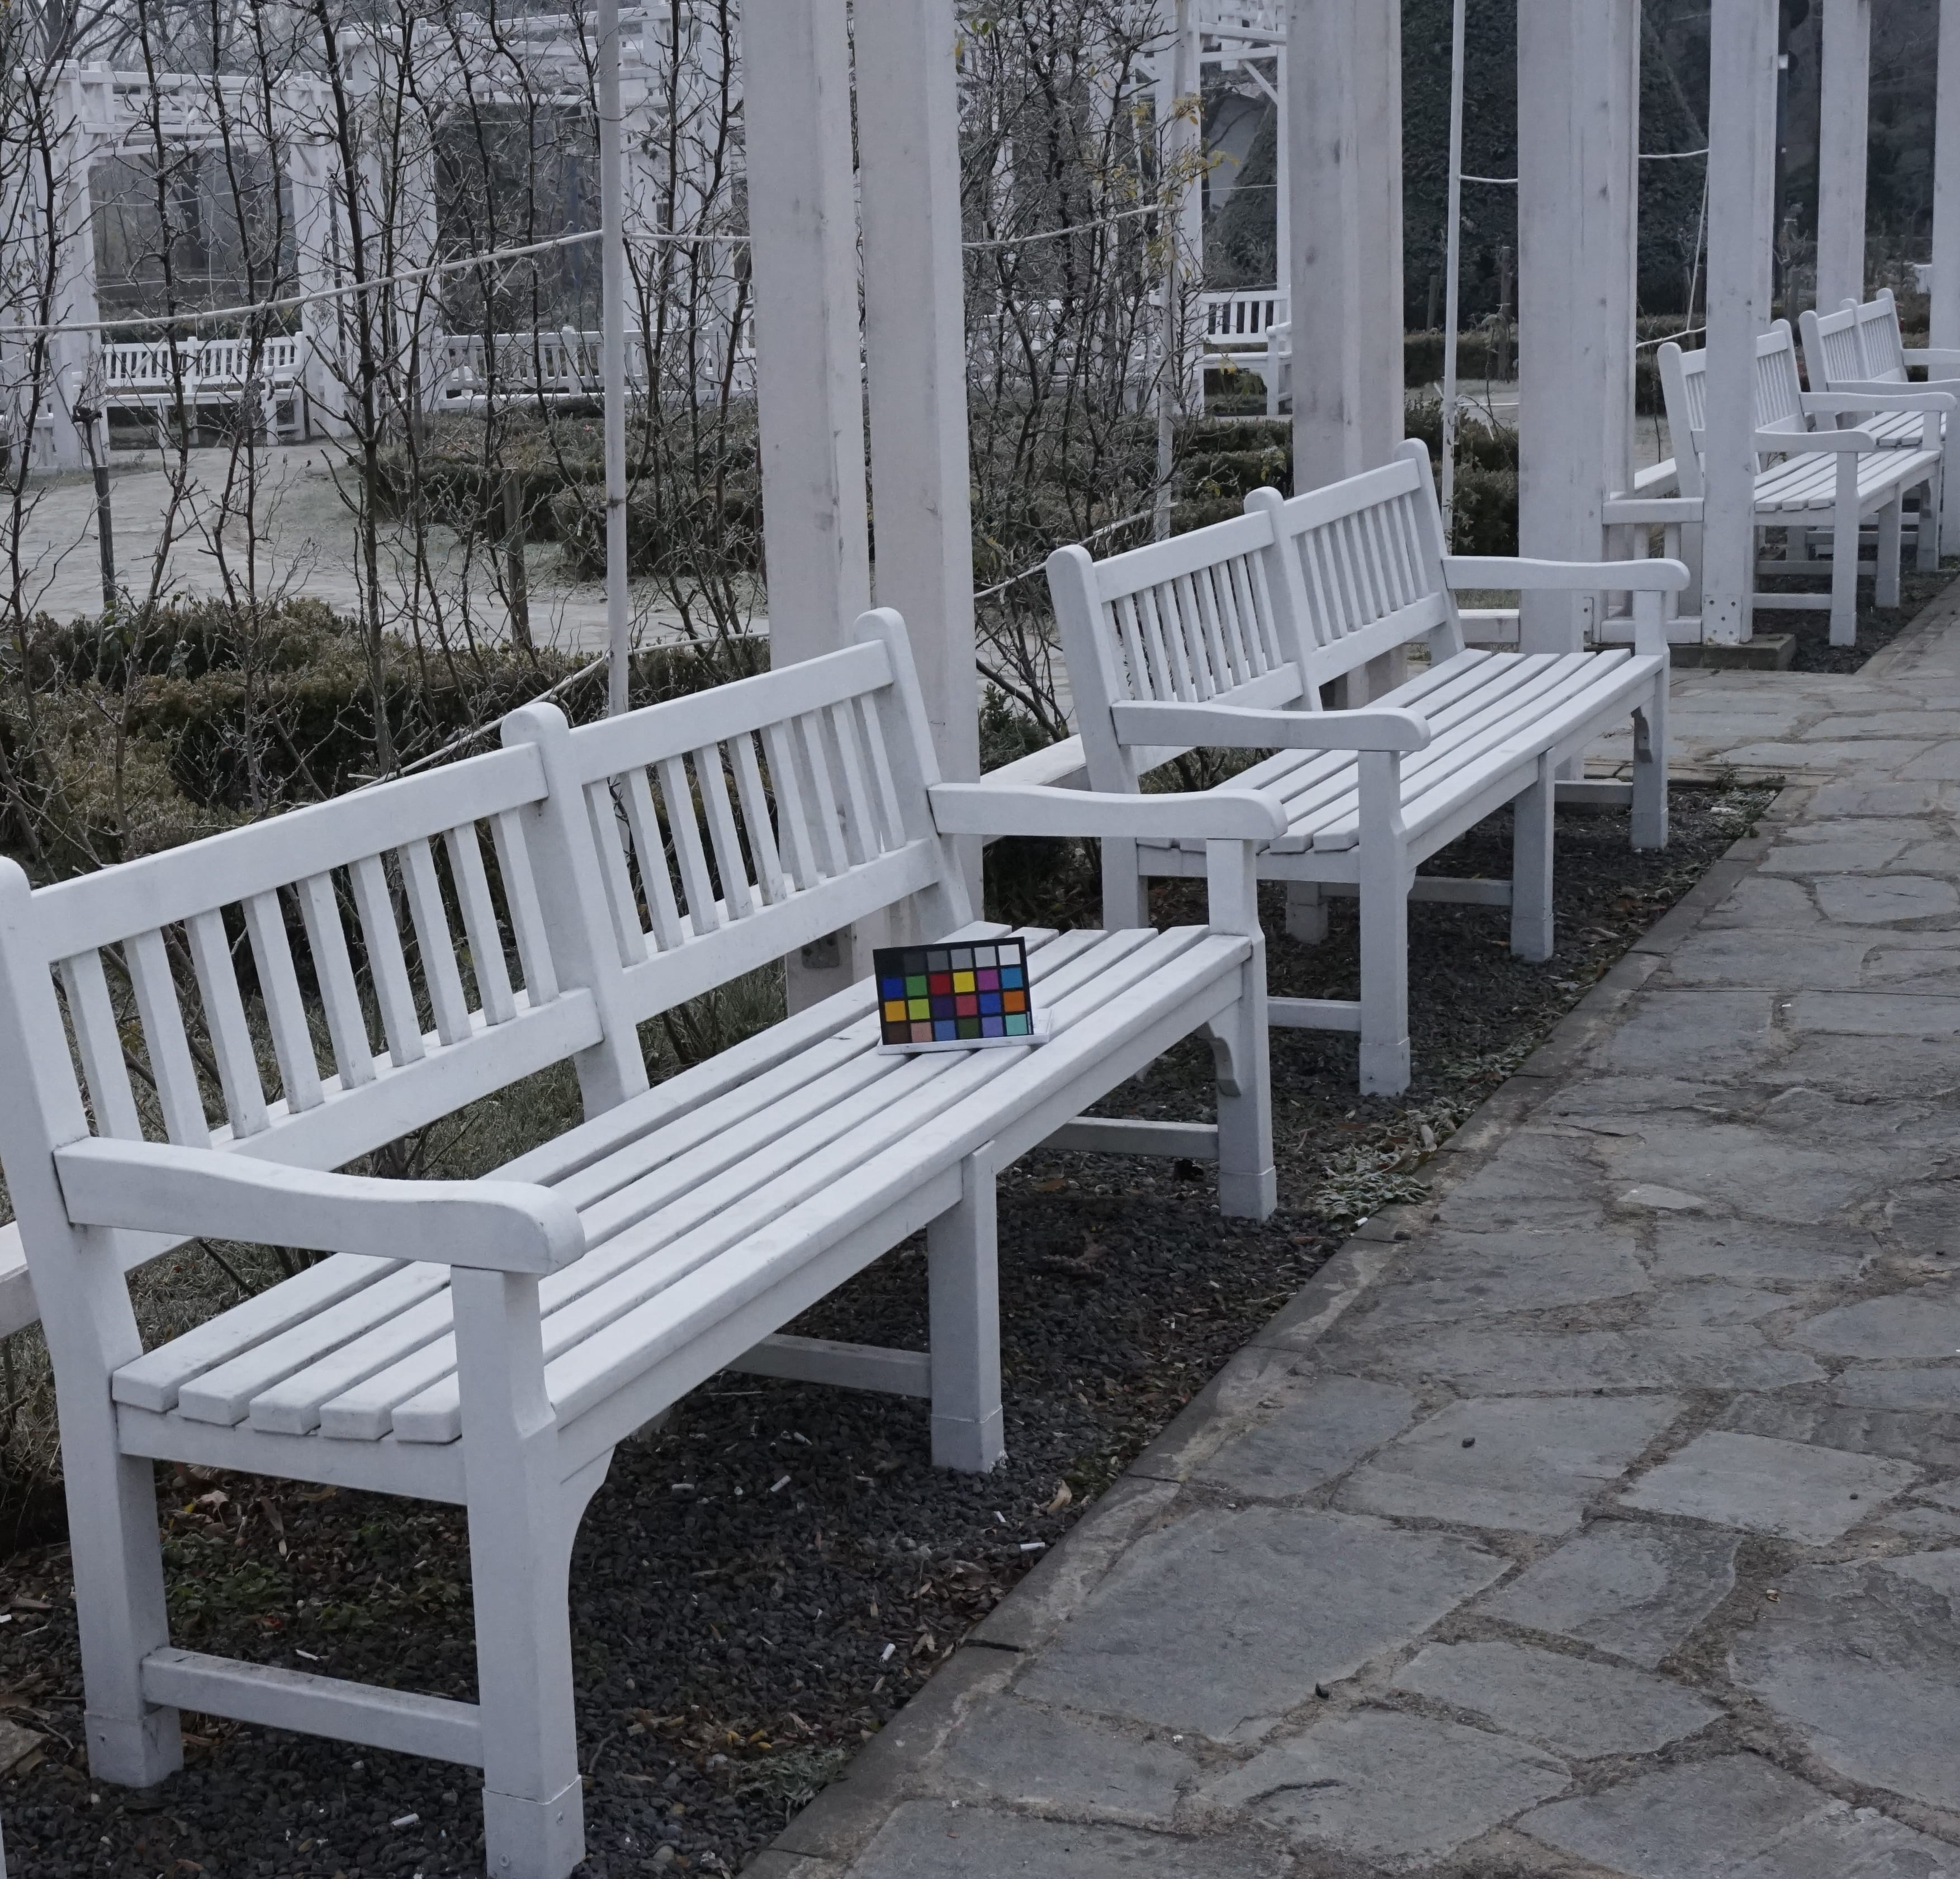
\includegraphics[height=4.2cm, width=4.2cm]{images/40_outdoor_GT.jpg}}  & 
 \subfloat[]{\label{set5-bic} 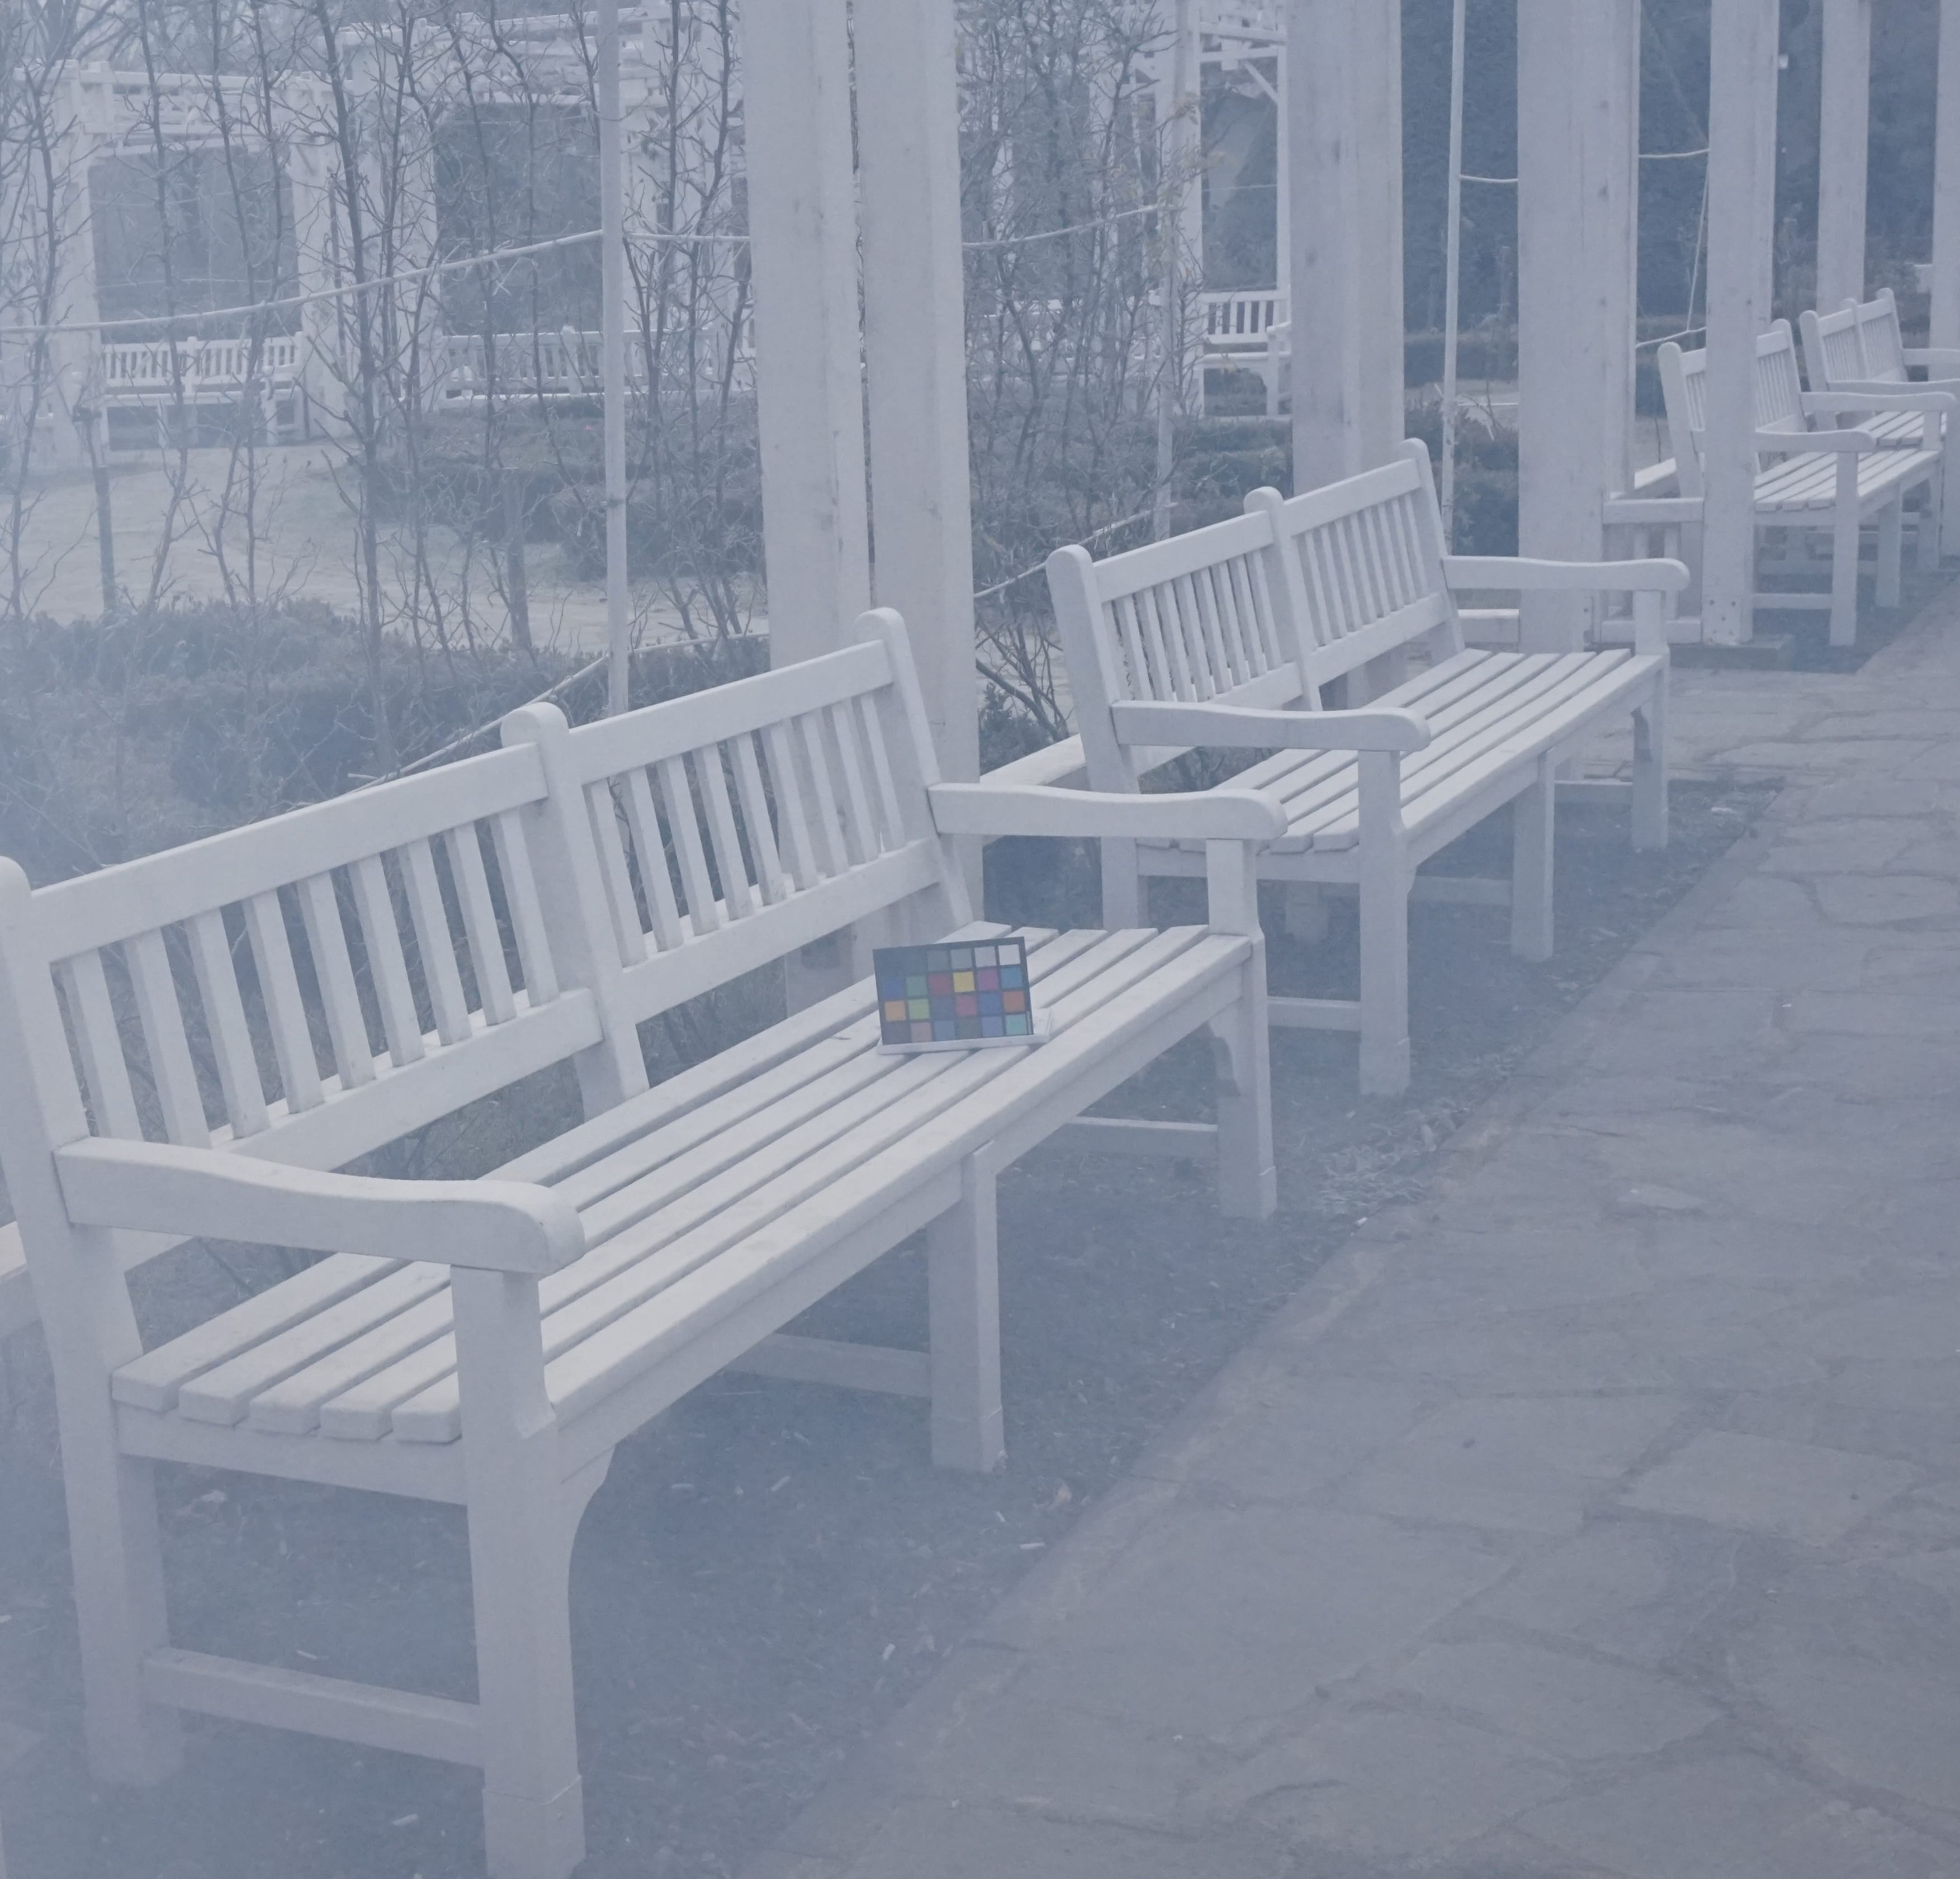
\includegraphics[height=4.2cm, width=4.2cm]{images/40_outdoor_hazy.jpg}} & 
  \subfloat[]{\label{set5-pred}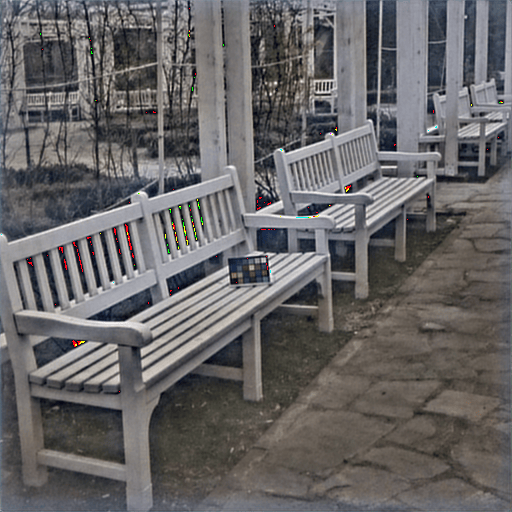
\includegraphics[height=4.2cm, width=4.2cm]{images/O-Dataset_40.png}} \\
 % \subfloat[]{\label{set14-or}\includegraphics[height=4.2cm, width=4.2cm]{images/GT22_dense.jpg}} & 
 %  \subfloat[] {\label{set14-bic}\includegraphics[height=4.2cm, width=4.2cm]{images/22_hazy.png}} & 
 %   \subfloat[]{\label{set14-pred}\includegraphics[height=4.2cm, width=4.2cm]{images/dense22.png}} \\
 \subfloat[] {\label{set14-org}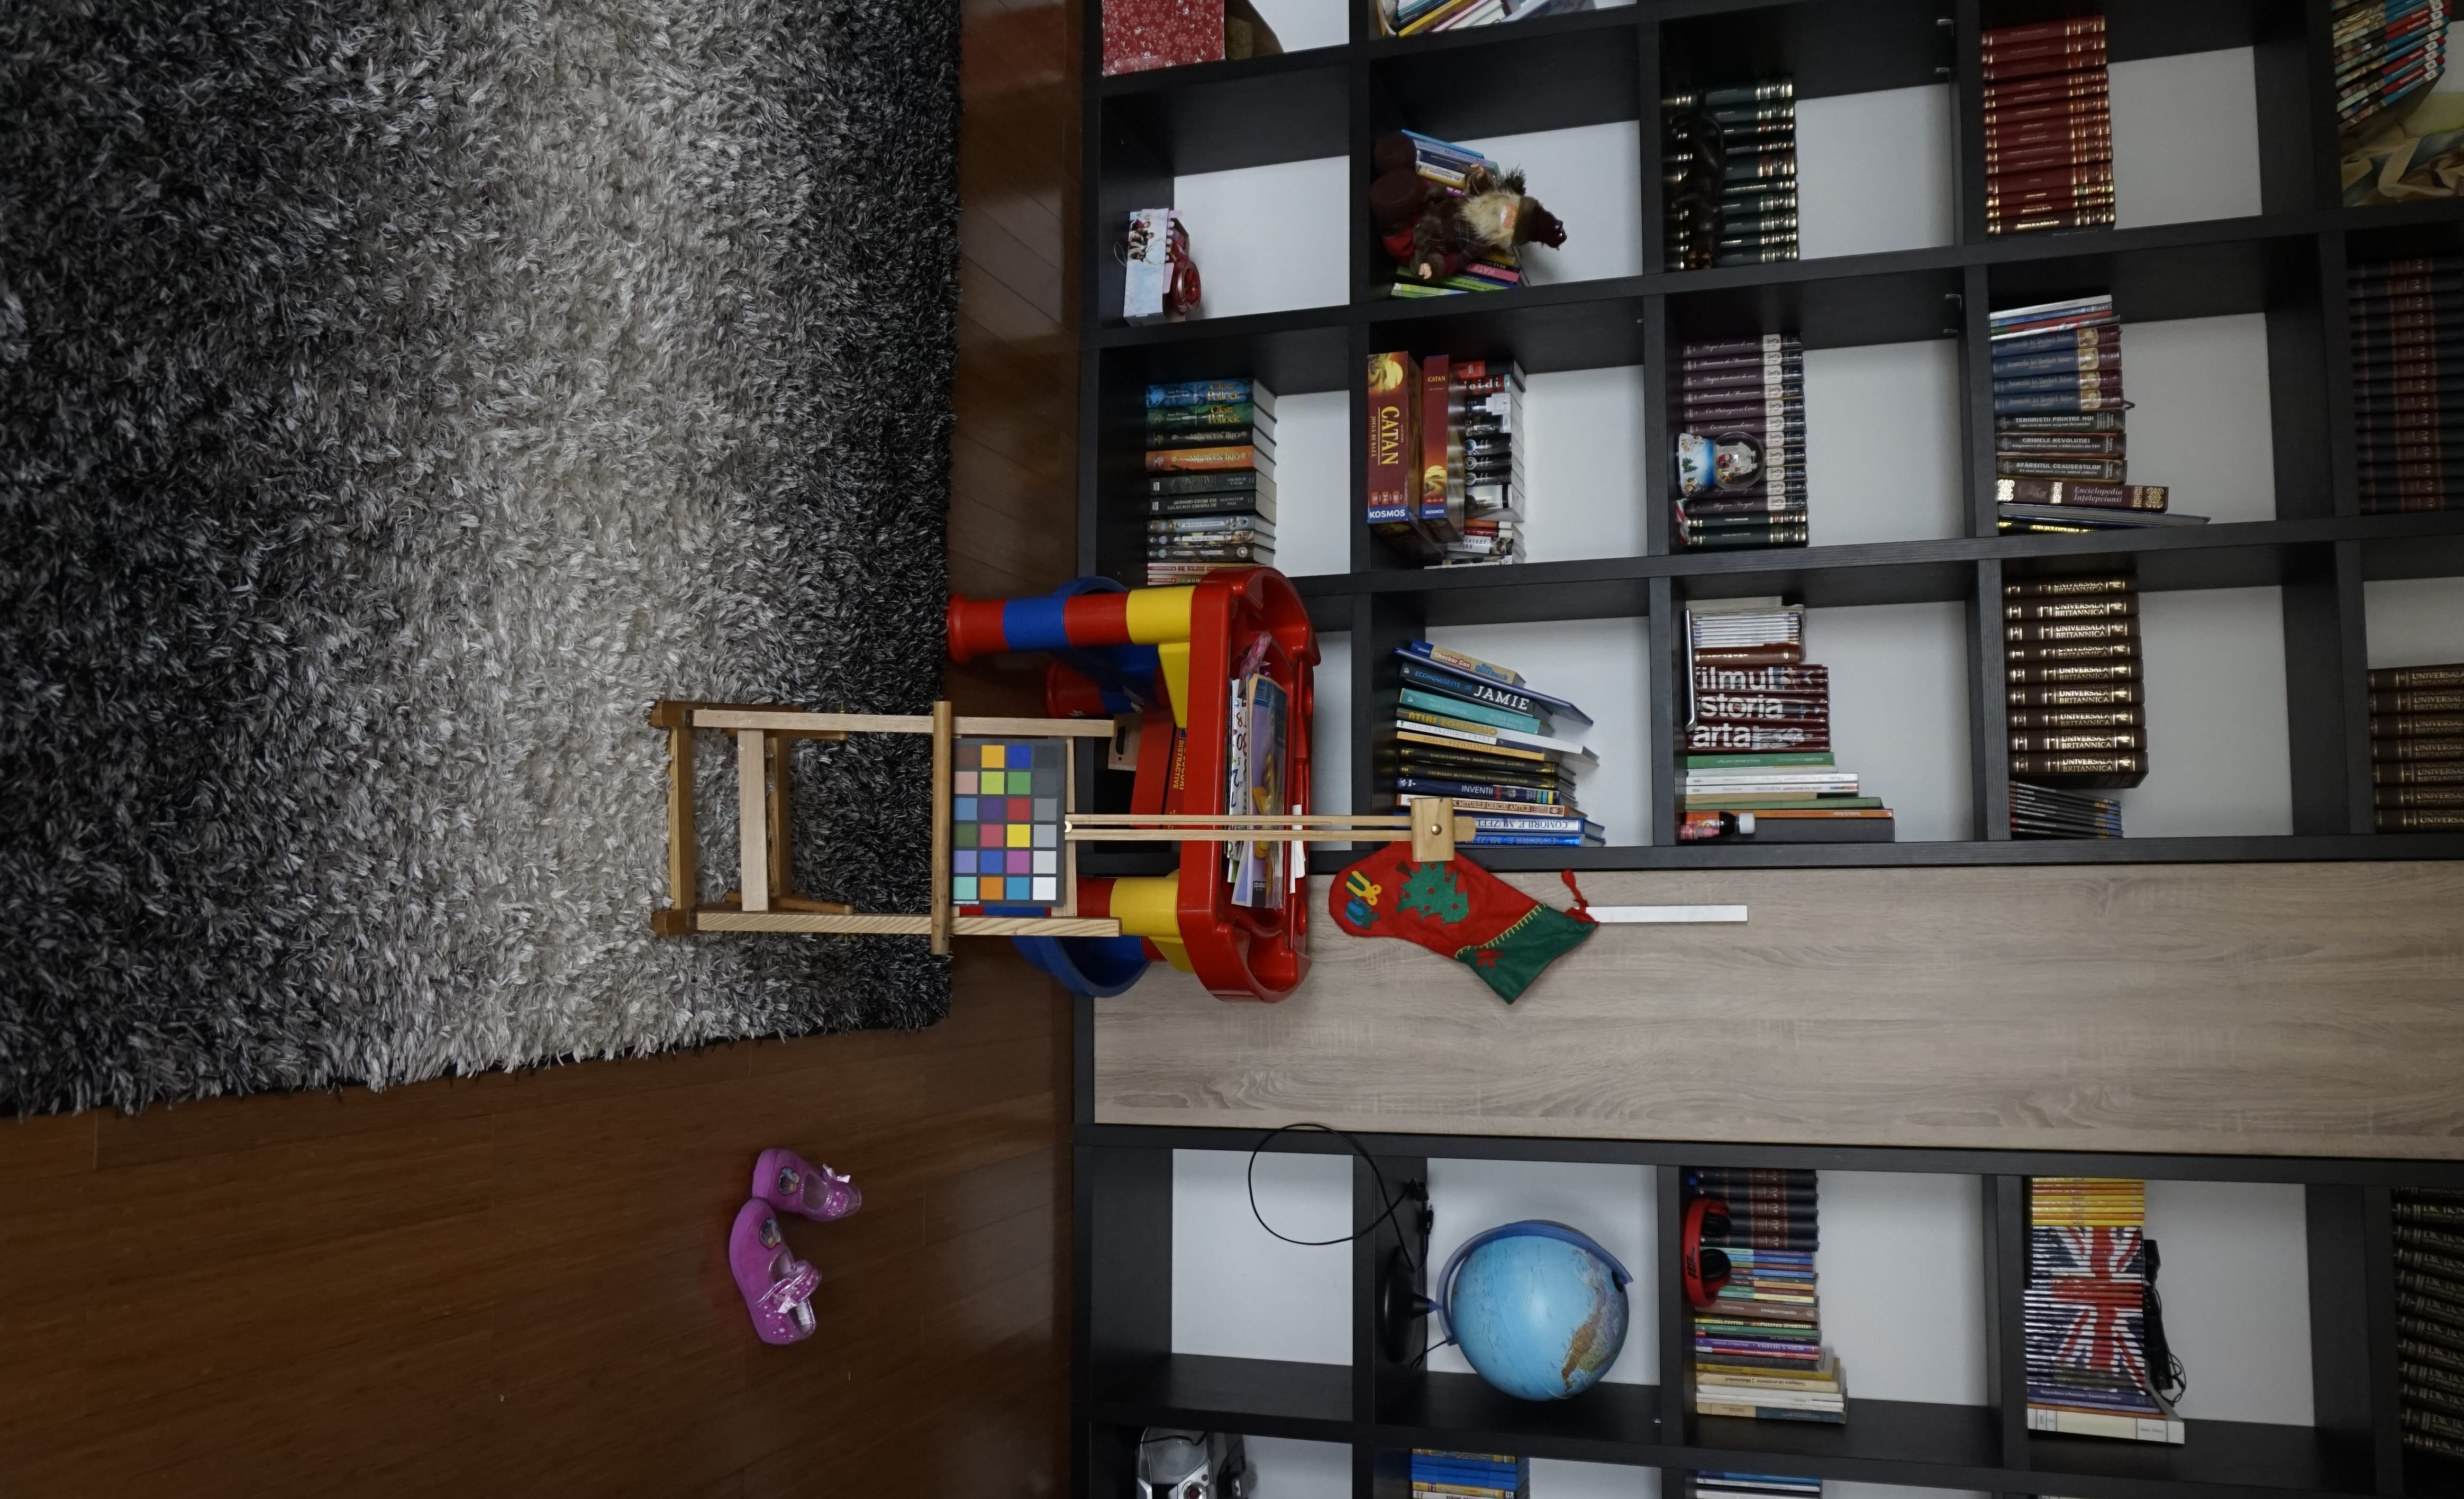
\includegraphics[height=4.2cm, width=4.2cm]{images/02_indoor_GT.jpg}} & 
 \subfloat[]{\label{set14-bicu} 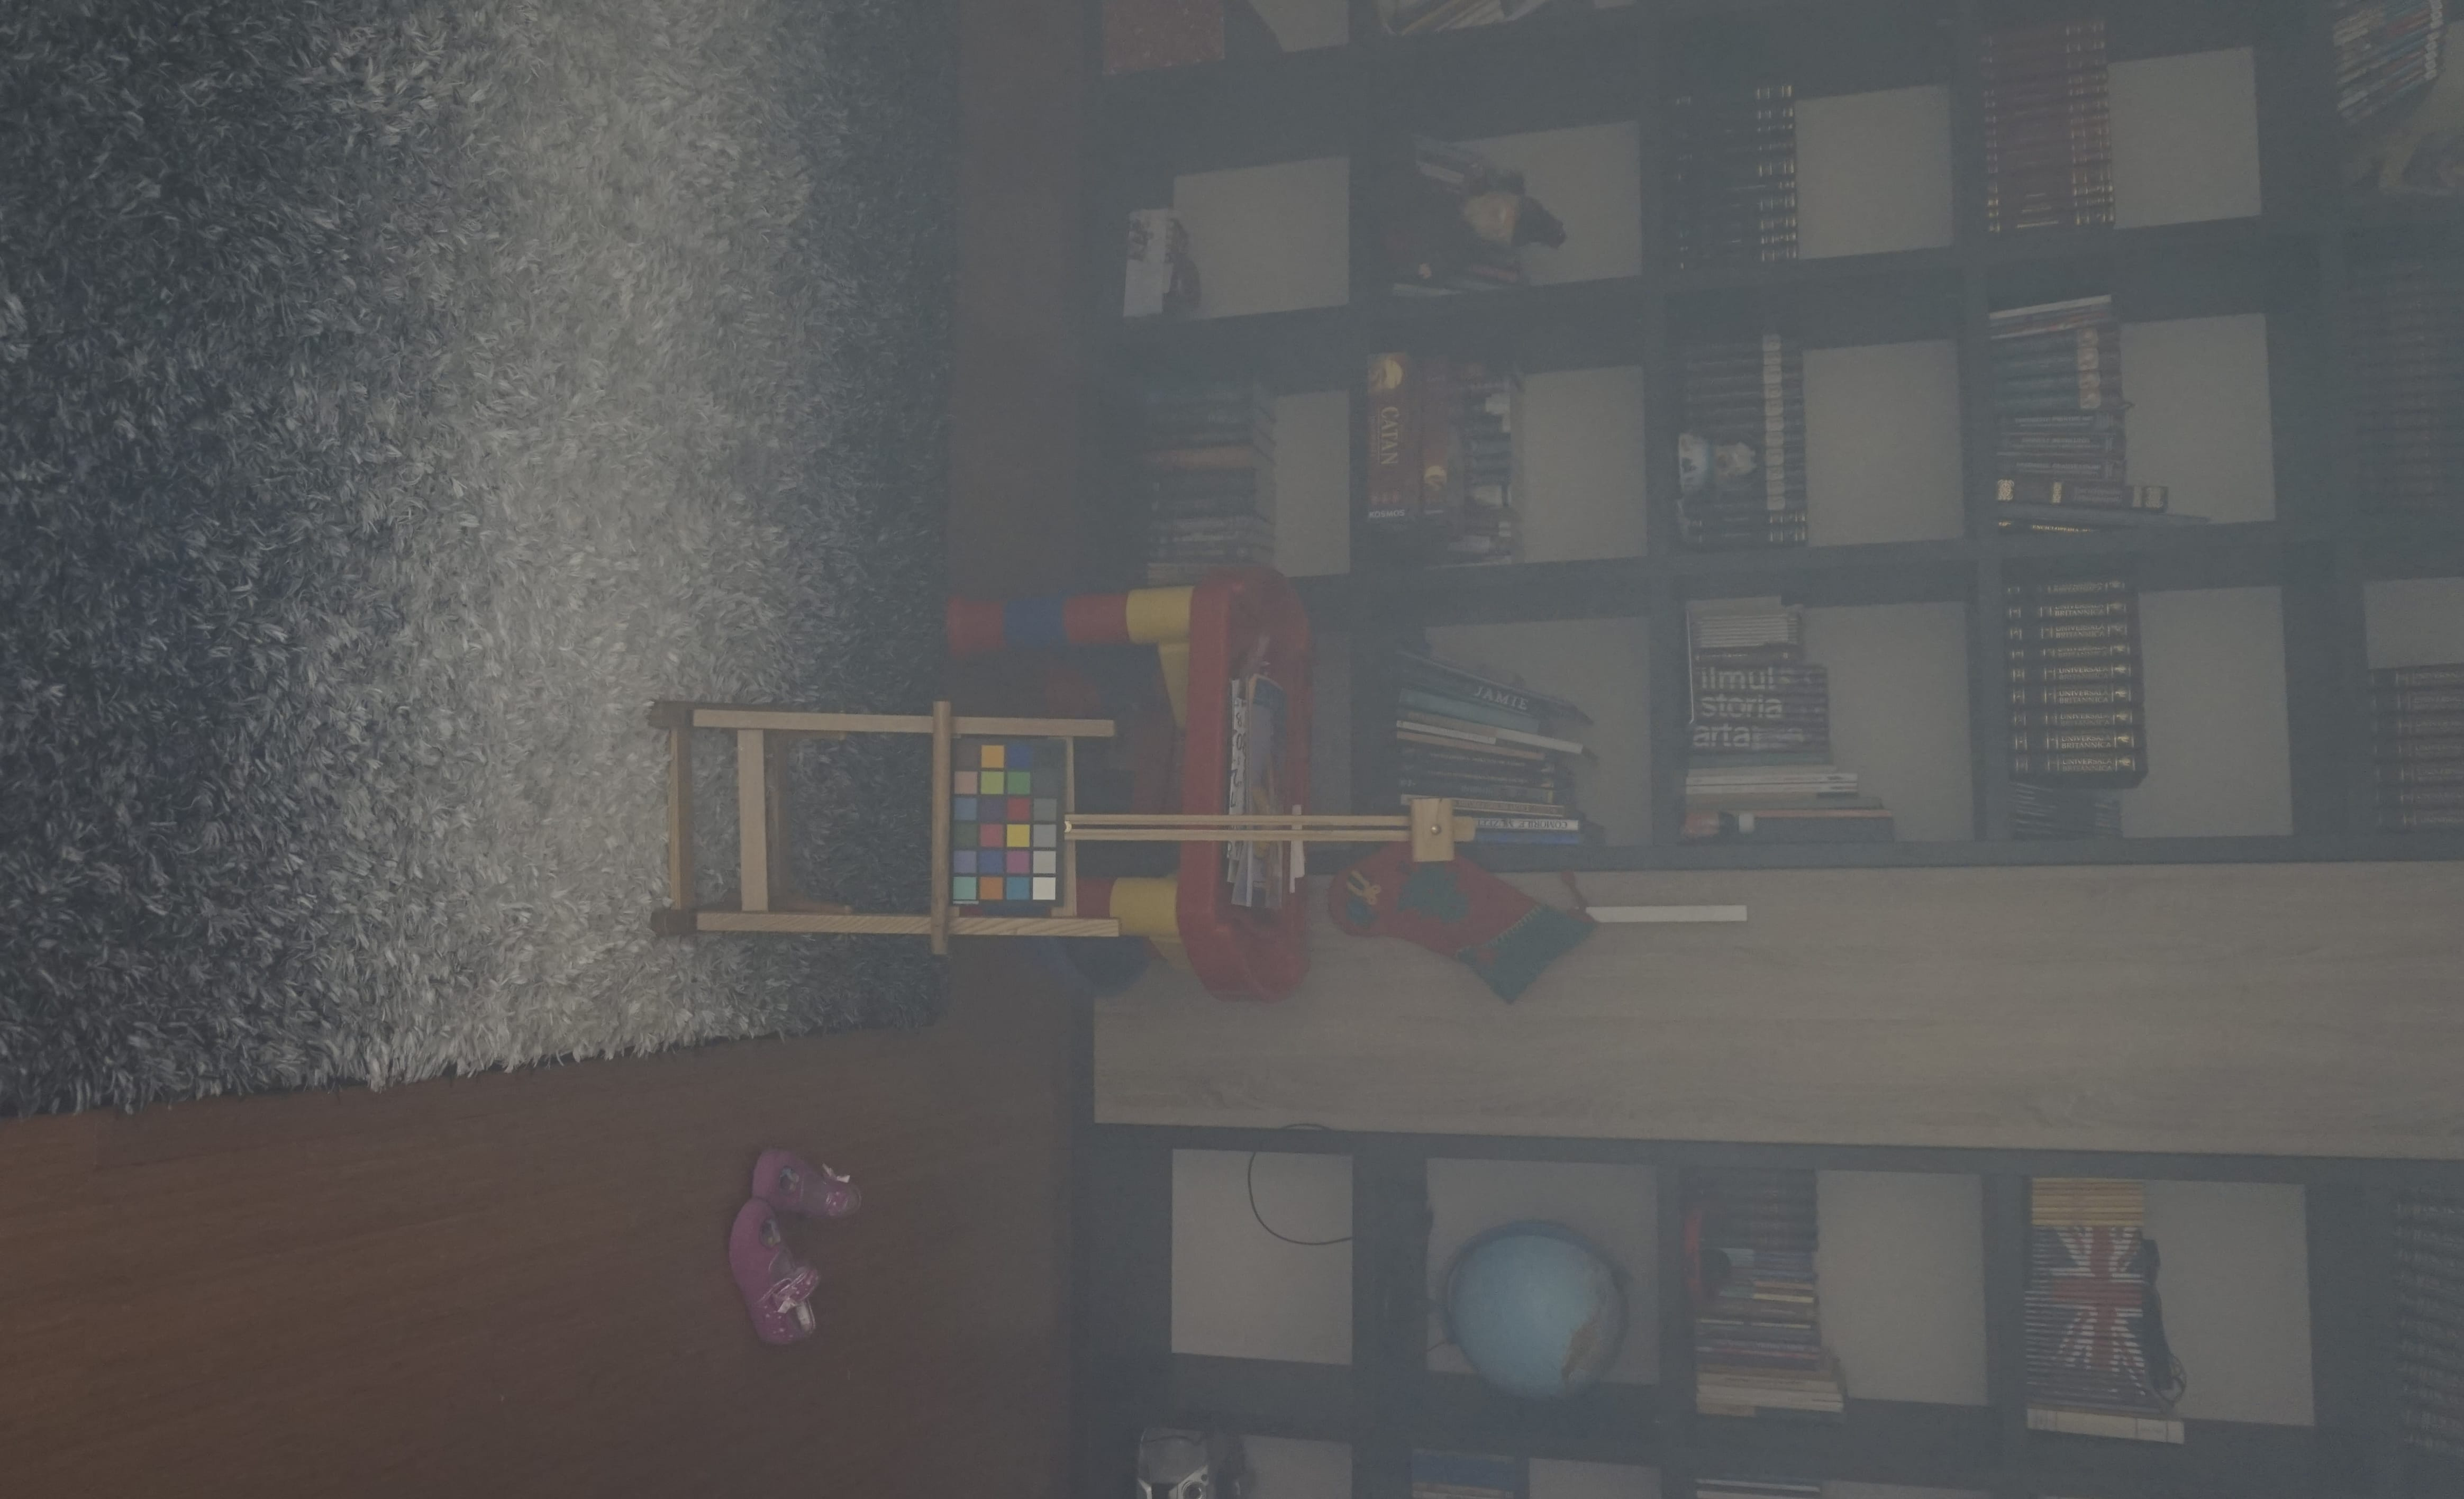
\includegraphics[height=4.2cm, width=4.2cm]{images/03_indoor_hazy.jpg}} & 
 \subfloat[]{\label{set14-predi} 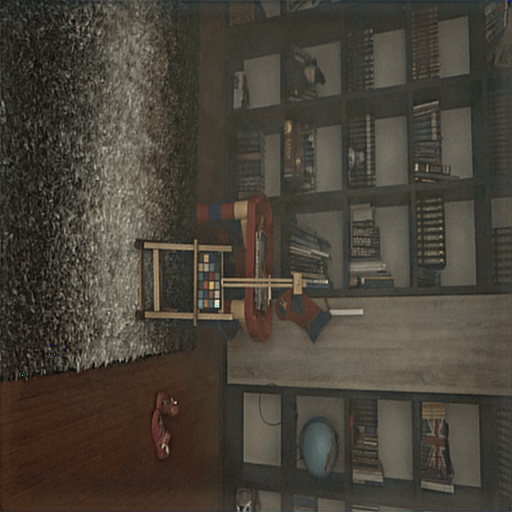
\includegraphics[height=4.2cm, width=4.2cm]{images/I-Dataset_2.png}} 

\end{tabular}
\label{tab:Results}
\end{figure*}

\subsection{Losses and metrics}\label{loss_metric}

The loss function associated with the trained model is stated as follows:
\begin{equation}
\mathcal{L} \ = \ \mathcal{L}_{{1, 2}} \ + \ \mathcal{L}_{FFT} \ + \ \mathcal{L}_{SSIM}
    \label{eqn:total_loss}
\end{equation}
\begin{itemize}
    \item Frequency-domain loss \cite{fft} ($\mathcal{L}_{FFT}$) transforms output images into frequency signals. To increase sharpness and
reduced noise and other artifacts. Let $m$, $n$ dimension of images $I_1$ and $I_2$ , where $K$ is
scaling factor
\textit{FFT} stands for \textit{Fast Fourier Transform} of Image $I$. The Fast Fourier transform is
\begin{equation}
    \mathcal{L}_{FFT} = \mathcal{L}^{\frac{m}{k}\times\frac{n}{k}} =  \frac{k^2}{m \times n} \left | FFT(I_1) - FFT(I_2) \right |^{\frac{m}{k}\times\frac{n}{k}}
    \label{eqn:fft}
\end{equation}
fast algorithm to compute $DFT$ i.e. \textit{Discrete Fourier Transform}. By transforming
images into frequency, we can learn to see the differences in higher dimensional region.
By transforming image signals into a frequency domain for Fourier transform such
that we can enhance the higher frequencies while keeping lower frequencies which will
sharpen the images. 
    \item Smooth $\mathcal{L}_{1}$ loss ($\mathcal{L}_{1}$) is amalgamation of $\mathcal{L}_{1}$ and $\mathcal{L}_{2}$ losses, when the respective 
absolute error is high it behaves like $\mathcal{L}_{1}$ and when the absolute error is close to zero it
behaves like an $\mathcal{L}_{2}$. We used Huber loss \cite{huber} as smooth $\mathcal{L}_{1}$ loss because of its similarity
\begin{equation}
    \mathcal{L}_{\delta}\left ( {a} \right ) \ = \ \left\{\begin{matrix}
{\frac{a^2}{2}} & for \ \left | a \right | \leq  \delta \\ \\
\delta \left ( \left | a \right |- \frac{\delta}{2} \right ) &  otherwise
\end{matrix}\right.
    \label{eqn:l1_loss}
\end{equation}
    \item Mean Square Error (\textit{MSE}) is used as $\mathcal{L}_{2}$ loss function as follows: \\
    
    \begin{equation}
    \mathcal{L}_{2}= \ MSE = \frac{1}{mn} \sum_{1}^{m} \sum_{1}^{n} \left \| \widehat I(n, m) - I^{*}(n, m)  \right \|^{2} 
     \label{eqn:mse}
\end{equation}
Where, $\widehat I$ is predicted image and $I^{*}$ is ground-truth image. 
    \item PSNR is used as a metric for image quality. The higher value indicates better quality. The unit of \textit{PSNR} is \texttt{dB}. We calcuate the \textit{PSNR} as following equation.
    \begin{equation}
    PSNR = 20 \log_{10} \left ( \frac{MAX_{ \widehat I}}{\sqrt{MSE}} \right )
    \label{eqn:psnr}
    \end{equation}
    Where, $\widehat I$ is predicted image based on \textit{MSE}  \eqref{eqn:mse}.
    \item Structural Similarity (\textit{SSIM}) is used as a metric to improve the structural accuracy of predicted output.
    \begin{equation}
        SSIM(x, y) \ = \ \frac{\left ( 2\mu_{x}\mu_{y} \ + \ C_{1} \right) \left ( 2\sigma_{xy} + \ C_{2} \right)}{\left ( \mu_{x}^{2} \ + \ \mu_{y}^{2} + C_{1} \right ) \left ( \sigma_{x}^{2} \ + \ \sigma_{y}^{2} + C_{2} \right )}
        \label{eqn:ssim}
    \end{equation}
     whereas, $\mu _{x}$ the pixel sample mean of x , $\mu _{y}$ the pixel sample mean of y, $\sigma _{x}^{2}$ and the change in variance of x, $\sigma _{y}^{2}$ can effect the variance of y, $\sigma_{xy}$ which is associated with the covariance of x,
     \item Structural Similarity loss ($\mathcal{L}_{SSIM}$) is used retain structural similarity of reconstructed image we minimized \textit{SSIM} loss. The loss function is stated as below,
     \begin{equation}
         \mathcal{L}_{SSIM} = \frac{\left ( 1- SSIM \right )}{2}
         \label{eqn:ssim_loss}
     \end{equation}
     where as \textit{SSIM} is from \eqref{eqn:ssim}
\end{itemize}


% Please add the following required packages to your document preamble:
% \usepackage{graphicx}
\begin{table}[h]
\caption{The quantitative  result of different traditional methods with our model on I-Haze, O-Haze.
}
\label{tab:my-table}
% \resizebox{\columnwidth}{!}{%
\begin{tabular}{cccccc}
\multicolumn{6}{c}{\textit{\textbf{I-Haze}}  \cite{i_haze} }                                   \\ \hline
\textbf{Metric} & \textit{\textbf{Berman et al.}} \cite{prior1} & \textit{\textbf{AOD-Net}} \cite{aod}  & \textbf{BPPNet} \cite{bppnet_sota} & \textit{\textbf{EDN-GTM}} \cite{sec_sota} & \textit{\textbf{Our}} \\ \hline
\textbf{PSNR (dB)} & 14.12  & 13.98  & 22.56           & \textbf{22.90}  & 22.54 \\
\textbf{SSIM}      & 0.6537 & 0.7323 & \textbf{0.8994} & 0.8270 & 0.8702         \\ \hline
\multicolumn{6}{l}{}                                                             \\
\multicolumn{6}{c}{\textit{\textbf{O-Haze}}  \cite{o_haze} }                                   \\ \hline
Metric          & \textbf{Berman et al.}   \cite{prior1}       & \textbf{AOD-Net}    \cite{aod}      & \textbf{BPPNet} \cite{bppnet_sota} & \textbf{EDN-GTM}  \cite{sec_sota}       & \textit{\textbf{Our}} \\ \hline
\textbf{PSNR (dB)} & 15.98  & 15.03  & \textbf{24.27}  & 23.46  & 23.02          \\
\textbf{SSIM}      & 0.5894 & 0.5385 & \textbf{0.8919} & 0.8198 & 0.8034         \\ \hline
\end{tabular}%
% }
\end{table}

\section{Experiments}
\label{experiments}


\subsection{Dataset}\label{dataset}
To train the model, we incorporated two different datasets Realistic Single Image Dehazing (\textit{RESIDE}) dataset \cite{bench} with  total number 18,200  images for training are consider and additionally the Real-world Video Dehazing dataset (\textit{REVIDE-indoor}) \cite{revid} with a total of 1697  images for training and 282 for testing. To infer the proposed model, we used various benchmarking datasets like Dense haze \cite{dense_haze}, NH haze \cite{nh_haze}, I haze \cite{i_haze} and O haze \cite{o_haze}. We split the training dataset into 80\% training and 20\% validation. In pre-processing, we resize input images into $128 \times 128$ and change the colour space to YCbCr. We used batch size $64$ for all of the images. 

\subsection{Training setup}\label{train_setup}

We used AdamW \cite{admw} rather than Adam optimizer, as we used weight normalization weight decay from AdamW will be a reasonable regularizer. The weights are initialized in uniform distribution as proposed by He et al. \cite{kaiming} initial biases were set to zero. The learning rate we consider for training the model is 0.0001 and the weight decay is $10^{-5}$. If the loss doesn't change for 7 epochs, then dynamically the learning rate will be reduced by a factor of 2.

After testing both $\mathcal{L}_1$ \eqref{eqn:l1_loss} and $\mathcal{L}_2$ losses \eqref{eqn:mse}, we choose $\mathcal{L}_2$ as our primary loss. The final loss function includes $\mathcal{L}_2$ loss, Frequency domain loss \eqref{eqn:fft}, and structural similarity loss \eqref{eqn:ssim_loss}, and metrics include PSNR \eqref{eqn:psnr} and SSIM \eqref{eqn:ssim} as shown in Fig  \eqref{tab:vis_loss_metric}.

% Please add the following required packages to your document preamble:
% \usepackage{graphicx}
\begin{figure}[h]
\caption{The training and validation plot. Blue (train) indicates training and orange (val) indicates validation. a) Loss, b) PSNR, c)SSIM}
\label{tab:vis_loss_metric}
\resizebox{\columnwidth}{!}{%
\begin{tabular}{lll}
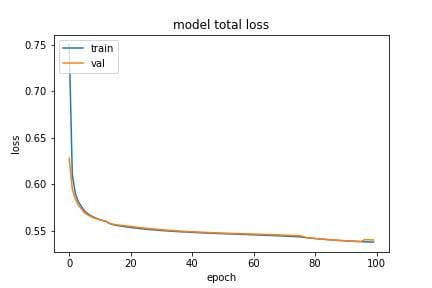
\includegraphics[height=14cm,width=16cm]{images/loss.jpg}& 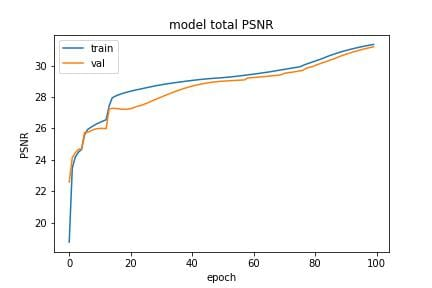
\includegraphics[height=14cm,width=16cm]{images/PSNR.jpg} & 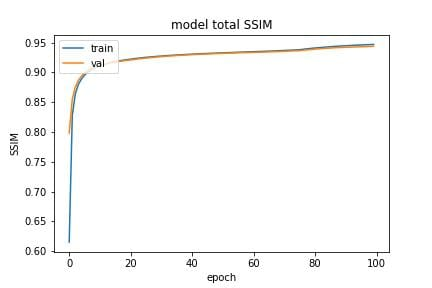
\includegraphics[height=14cm, width=16cm]{images/SSIM.jpg} \\
\multicolumn{1}{c} {\Huge{a) Loss}} & \multicolumn{1}{c}{\Huge{b) PSNR}} & \multicolumn{1}{c}{\Huge{c) SSIM}}
\end{tabular}%
}
\end{figure}

\subsection{Comparing results with other methods}
\label{comapring}
We computed metrics PSNR \eqref{eqn:psnr} and SSIM \eqref{eqn:ssim} on various real-world and synthetic images. We presented our results in  Table.~\eqref{tab:my-table} and Table. \eqref{tab:my-table1} with a detail analysis with existing methods.
\label{comparing}

\begin{table}[h]
\centering
\caption{The quantitative analysis of result  with respect to the existing  methods and our model on Dense-Haze, NH-Haze.
}
\label{tab:my-table1}
% \resizebox{\columnwidth}{!}{%
\begin{tabular}{cccccc}
\multicolumn{6}{c}{\textit{\textbf{Dense-Haze}}   \cite{dense_haze} }                                      \\ \hline
\textbf{Metric} & \textit{\textbf{Berman et al.}} \cite{prior1} & \textit{\textbf{AOD-Net}} \cite{aod} & \textbf{BPPNet} \cite{bppnet_sota} & \textit{\textbf{EDN-GTM}} \cite{sec_sota} & \textit{\textbf{Our}} \\ \hline
\textbf{PSNR (dB)} & 13.18 & 13.14       & 17.01       & 15.43          & \textbf{17.60} \\
\textbf{SSIM}      & 0.358 & 0.414       & 0.613       & 0.520          & \textbf{0.716} \\ \hline
\multicolumn{6}{l}{}                                                                     \\
\multicolumn{6}{c}{\textit{\textbf{NH-Haze}}  \cite{nh_haze}}                                           \\ \hline
Metric          & \textbf{He et al.}  \cite{he}            & \multicolumn{2}{c}{\textbf{AOD-Net} \cite{aod}}       & \textbf{EDN-GTM} \cite{sec_sota}         & \textit{\textbf{Our}} \\ \hline
\textbf{PSNR (dB)} & 16.62 & \multicolumn{2}{c}{15.40} & \textbf{20.24} & 18.93          \\
\textbf{SSIM}      & 0.523 & \multicolumn{2}{c}{0.569} & 0.718          & \textbf{0.746} \\ \hline
\end{tabular}%
% }
\end{table}
As exhibited in Table \eqref{tab:my-table}, the model performs near state-of-the-art in both PSNR and SSIM metrics on both datasetes \cite{i_haze, o_haze}. Whereas from Table \eqref{tab:my-table1}, our model outperforms existing methods in both PSNR and SSIM with the Dense-haze dataset \cite{dense_haze}. For the NH-Haze \cite{nh_haze} dataset, our model outperforms existing models in SSIM and the PSNR difference between our model and the existing model is 1.31dB. In both cases, EDN-GTM \cite{sec_sota} struggles in the SSIM metric, but our method gives a precise SSIM score because of the Structural similarity loss \eqref{eqn:ssim_loss}, see results in Fig (\ref{tab:Results}).

\section{Ablation study}
\label{ablation study}
We conducted an ablation study on I-Haze, O-Haze, Dense-Haze and NH-haze datasets.  We evaluated ablation with loss components in Section \ref{loss_ablation} and colourspace image representation in training images in Section \ref{ycbcr_vs_rgb}.
\subsection{Loss ablation}
\label{loss_ablation}
In section \ref{loss_metric}, we used three types of losses to train our neural network. In this section, we will assess the result if we change the loss function $\mathcal{L}_2$ with $\mathcal{L}_1$, i.e. Huber loss. Our observation is presented in Table \eqref{tab:l1vl2}, which shows the qualitative comparison between these losses.
% Please add the following required packages to your document preamble:
% \usepackage{graphicx}
\begin{table}[h]
\caption{The quantitative comparison result of $\mathcal{L}_1$ verses $\mathcal{L}_2$ on I-Haze, O-Haze, Dense-Haze and NH-Haze.}
    \label{tab:l1vl2}
\centering
    \begin{tabular}{ccccc}
        \multicolumn{5}{c}{\textit{\textbf{A) $\mathcal{L}_1$ Loss}}}   \\ \hline
        \textbf{Metric} & \textit{\textbf{I-Haze}} \cite{i_haze} & \textit{\textbf{O-Haze}} \cite{o_haze} & \textbf{Dense-Haze} \cite{dense_haze} & \textit{\textbf{NH-Haze}} \cite{nh_haze} \\ \hline
        \textbf{PSNR (dB)} & 21.41 & 21.24 & 17.44 & 17.78 \\
        \textbf{SSIM}      & 0.843 & 0.779 & 0.697 & 0.713 \\ \hline
        \multicolumn{5}{l}{}                               \\
        \multicolumn{5}{c}{\textit{\textbf{B) $\mathcal{L}_2$ Loss}}}   \\ \hline
        \textbf{Metric} & \textit{\textbf{I-Haze}} \cite{i_haze} & \textit{\textbf{O-Haze}} \cite{o_haze} & \textbf{Dense-Haze} \cite{dense_haze} & \textit{\textbf{NH-Haze}} \cite{nh_haze}        \\ \hline
        \textbf{PSNR (dB)} & 22.54 & 23.02 & 17.60 & 18.93 \\
        \textbf{SSIM}      & 0.870 & 0.803 & 0.716 & 0.746 \\ \hline
    \end{tabular}
\end{table}

\subsection{Use of YCbCr versus RGB space}
\label{ycbcr_vs_rgb}
In Section \ref{color_space}, we discussed the use of YCbCr colourspace over RGB. In this section, we will examine the qualitative results of both colourspace image representations for training the proposed network. Our findings reveal that the YCbCr colourspace images give slightly better results than the RGB colourspace images in most of the datasets. On some input images, RGB-based images were perceptually better than the YCbCr. Also, the metric-wise difference is diminutive for all datasets.


\section{Conclusion}
\label{conclusion}
We presented the coherent architecture train on sufficiently large and diverse data that can give near state-of-the-art results on indoor, outdoor, non-homogenous, dense and synthetic haze environments on qualitative metrics PSNR and SSIM. Our model gives structurally enhanced output on poorly visible input images. We used a combination of loss functions to generate a haze-free image without colour degradation, noise and structural loss. Our method demonstrated by choosing adequate qualitative and quantitative data miniature and straightforward network can effective as the existing methods. In future, our model can be used to get haze-free images for vision tasks such as object detection,  segmentation and human action recognition if needed. Also, we will improve our model on low-light hazy images and colour restoration from densely hazy images.
\vspace{12pt}


% \bibstyle{bst/sn-mathphys.bst}
\bibliography{HAze}
\end{document}
